\chapter{Feature Visualization}

Feature Visualization is a technique that involves maximizing values of neurons, sets of neurons or even layers of a Neural Network in order to understand concepts learned by the model.
By maximizing a neuron's value, we can better understand what set of features each part of our network is learning to capture and verify if the network is aligned with human judgement.
In simple terms, Feature Visualization can be described by the following optimization problem:

\begin{equation}
    \text{img}^* = \argmax_{\text{img}} h_{n, x, y, z} (\text{img})
    \label{eq:feat_vis_optimization}
\end{equation}

\noindent where \(h\) represents the activation of a neuron, img is the input of the network, \(x\) and \(y\) represent the spatial position of the neuron, \(n\) is the layer of the network and \(z\) is the channel index.
This expressions represents the problem of maximizing a value of a single neuron. For a set of neurons, the problem can be described as the formula:

\begin{equation}
    \text{img}^* =  \argmax_{\text{img}} \mathlarger{\mathlarger{\sum}}_{(n, x, y, z) \: \in \: A} \!\!\! h_{n, x, y, z} (\text{img})
    \label{eq:feat_vis_optimization_multivar}
\end{equation}

where \(A \subseteq \mathbb{N}^4\) is a set of combinations of network layer, channel index and spatial position vectors.

In order to find a solution to the optimization problem, we can use the Gradient Descent technique presented in \hyperref[sec:gradient_descent]{Chapter 1}.
However, instead of minimizing an optimization problem, we are looking for a solution that maximizes \hyperref[eq:feat_vis_optimization]{Equation 3.1} or \hyperref[eq:feat_vis_optimization_multivar]{Equation 3.2}.
Therefore, instead of subtracting the partial derivative term of \hyperref[eq:gradient_descent]{Equation 1.2} we just need to add the partial derivative multiplied by the \emph{learning rate} (We will call the technique \emph{Gradient Ascent}). 
Thus, the following formula is derived for Feature Visualization:

\begin{equation}
    \text{img}_{t + 1} = \text{img}_t + \eta \: \mathlarger{\mathlarger{\sum}}_{(n, x, y, z) \: \in \: A} \frac{\mathlarger{\mathlarger{\partial}} h_{n, x, y, z} (\text{img}_t)}{\mathlarger{\mathlarger{\partial}} \text{img}_t}
    \label{eq:feat_vis_formula}
\end{equation}

\noindent where \(t\) is the iteration \(t\) of the algorithm. 

The initial image img\(_0\) can be defined in two ways:

\begin{itemize}
    \item A completely random initialization, with img\(_0(c, x, y) = U[0, 1]\) for each channel \(c\) and image spatial positions \(x\) and \(y\).
    \item A user defined image, normally a real world image.
\end{itemize}

The choice between these two approaches depends on the researcher's ultimate objective when using the algorithm.
Providing an initial non-random image allows researchers to focus on specific features within the image and examine their effects on a particular set of neurons. 
In contrast, using a random image may be better suited for discovering unknown features.

Like most optimization problems, the Feature Visualization problem doesn't strictly have a single optimal solution, but rather multiple viable solutions that maximize the given set of neurons.
For example, a set of seemingly random images may activate a neuron fully while at the same time an image of a cute dog may also activate this same neuron to its maximum value.
Directly applying \emph{Gradient Ascent} to random images without additional techniques often produces images that poorly align with human perception. This outcome occurs not because human-aligned images fail to maximize the neuron's value, but because solutions comprising seemingly random pixels are closer to the image's initial state.

% TODO: Acho que seria legal colocar por aqui uma imagem aleatória e a mesma imagem com feature visualization usando diretamente apenas Gradient Ascent, sem piramides
\begin{figure}
    \captionsetup{justification=centering}

    \begin{subfigure}[t]{0.28\textwidth}
        \captionsetup{justification=centering}
        \centering
        
\includegraphics[width=.7\linewidth]{figuras/random_image.png}
        \caption{Original Image}
    \end{subfigure}
    \hfill
    \begin{subfigure}[t]{0.28\textwidth}
        \captionsetup{justification=centering}
        \centering
        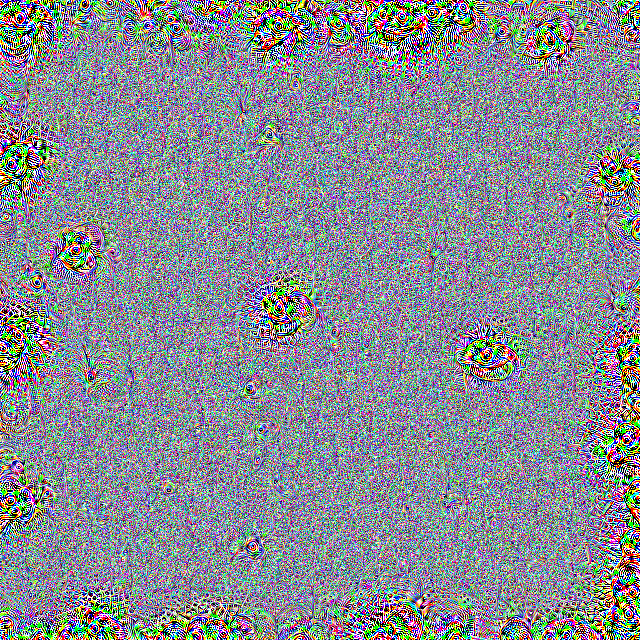
\includegraphics[width=.7\linewidth]{figuras/random_image_dream.png}
        \caption{Feature Visualization of Convolution layer 22 of VGG16}
    \end{subfigure}
    \hfill
    \begin{subfigure}[t]{0.28\textwidth}
        \captionsetup{justification=centering}
        \centering
        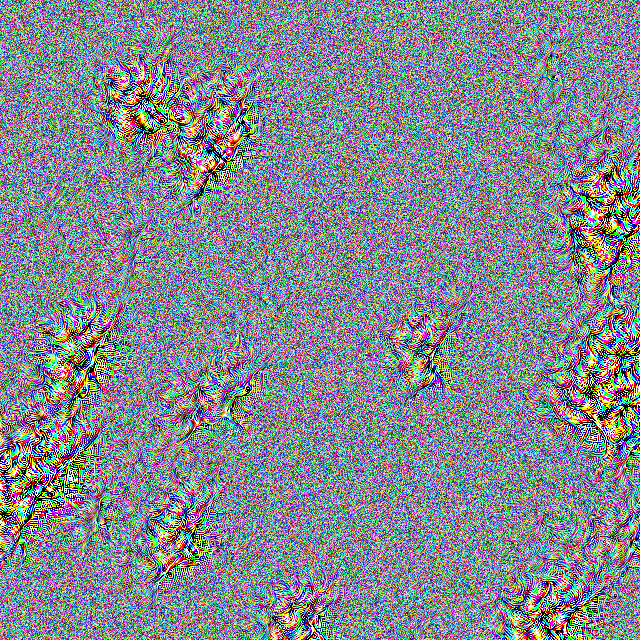
\includegraphics[width=.7\linewidth]{figuras/random_image_dream_class_250.png}
        \caption{Feature Visualization of Siberian Husky (IMAGENET index 250) neuron of VGG16}
    \end{subfigure}

    \caption{
        Feature Visualization images using solely Gradient Ascent. 
    Little human-recognizable features are present in the resulting images
    }
\end{figure}

To identify human-aligned features in our models, we need effective techniques for generating images that closely correspond to those features. 
A closer examination reveals that Feature Visualization using solely Gradient Ascent typically produces features that occupy only small portions of the final image.

To expand these features across a larger area and create more intricate forms, we can downscale the image and apply the Gradient Ascent step. 
Once the downscaled image has been refined, it can be upscaled by a specific factor, and Gradient Ascent can be reapplied. 
\newpage
\noindent
Repeating this process until the image reaches its original size enables the generation of more detailed and compelling results, as demonstrated below:

\begin{figure}
    \captionsetup{justification=centering}

    \begin{subfigure}[t]{0.45\textwidth}
        \captionsetup{justification=centering}
        \centering
        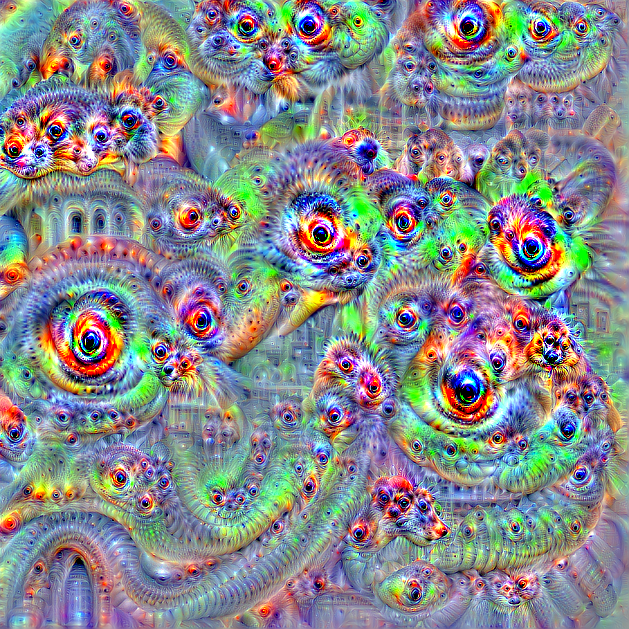
\includegraphics[width=.7\linewidth]{figuras/random_image_dream_pyramid.png}
        \caption{Feature Visualization of Convolution layer 22 of VGG16}
        \label{fig:feat_conv_L22_pyramid}
    \end{subfigure}
    \hfill
    \begin{subfigure}[t]{0.45\textwidth}
        \captionsetup{justification=centering}
        \centering
        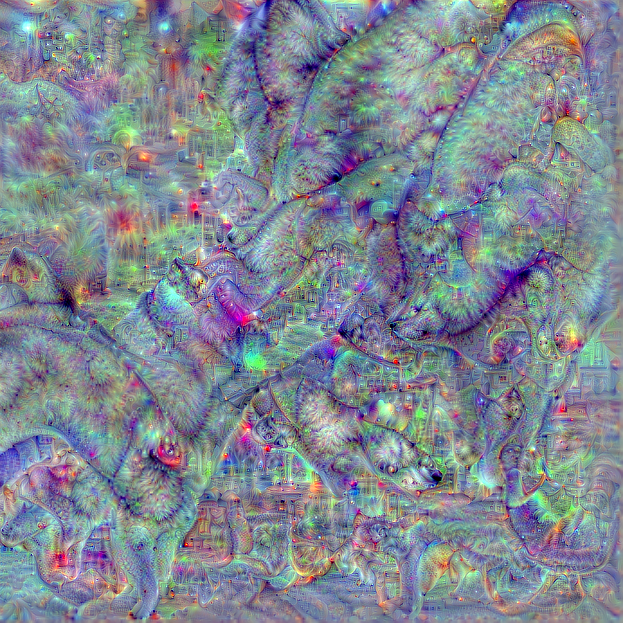
\includegraphics[width=.7\linewidth]{figuras/random_image_dream_pyramid_class_250.png}
        \caption{Feature Visualization of Siberian Husky (IMAGENET index 250) neuron of VGG16}
        \label{fig:feat_conv_I250_pyramid}
    \end{subfigure}

    \caption{By employing Gradient Ascent across multiple image scales, we achieve results that align more closely with human perception. In Figure \ref{fig:feat_conv_L22_pyramid}, eye-like structures frequently emerge in the generated images, while in Figure \ref{fig:feat_conv_I250_pyramid}, fur-like textures dominate—patterns strongly reminiscent of a Siberian Husky's coat.}
\end{figure}